Advances in artificial intelligence (AI) have resulted in the development of highly capable AI systems that make decisions for reasons we do not understand. This has caused concern that AI systems that we cannot trust are being widely deployed in the economy and in our lives, introducing a number of novel risks \citep{hendrycks2023overview}, including potential future risks that AIs might deceive humans in order to accomplish undesirable goals \citep{ngo2022alignment}. Mechanistic interpretability seeks to mitigate such risks through understanding how neural networks calculate their outputs, allowing us to reverse engineer parts of their internal processes and make targeted changes to them \citep{cammarata2021curve, wang2022interpretability, elhage2021mathematical}.

To reverse engineer a neural network, it is necessary to break it down into smaller units (features) that can be analysed in isolation. Using individual neurons as these units has had some success \citep{olah2020zoom, bills2023language}, but a key challenge has been that neurons are often \textit{polysemantic}, activating for several unrelated types of feature \citep{olah2020zoom}. Also, for some types of network activations, such as the residual stream of a transformer, there is little reason to expect features to align with the neuron basis \citep{elhage2023privileged}.

\citet{elhage2022toy} investigate why polysemanticity might arise and hypothesise that it may result from models learning more distinct features than there are dimensions in the layer. They call this phenomenon \textit{superposition}. Since a vector space can only have as many orthogonal vectors as it has dimensions, this means the network would learn an overcomplete basis of non-orthogonal features. Features must be sufficiently sparsely activating for superposition to arise because, without high sparsity, interference between non-orthogonal features prevents any performance gain from superposition. This suggests that we may be able to recover the network's features by finding a set of directions in activation space such that each activation vector can be reconstructed from a sparse linear combinations of these directions. This is equivalent to the well-known problem of sparse dictionary learning  \citep{olshausen1997sparse}. 

% Building on \citet{sharkey2023technical}, we train sparse autoencoders to learn these sets of directions. Our approach is also similar to \citet{yun2021transformer}, who apply sparse dictionary learning to all residual stream layers in a language model simultaneously, and forthcoming work by Anthropic, who apply this method to a custom 1-layer transformer \citep{anthropic2023}. Our method is summarised in Figure \ref{fig:overview} and described in Section \ref{section:dictionary_learning}.

Building on \citet{sharkey2023technical}, we train sparse autoencoders to learn these sets of directions. Our approach is also similar to \citet{yun2021transformer}, who apply sparse dictionary learning to all residual stream layers in a language model simultaneously. Our method is summarised in Figure \ref{fig:overview} and described in Section \ref{section:dictionary_learning}.

We then use several techniques to verify that our learned features represent a semantically meaningful decomposition of the activation space. First, we show that our features are on average more interpretable than neurons and other matrix decomposition techniques, as measured by autointerpretability scores (Section \ref{section:autointerp}) \citep{bills2023language}. We then run case studies on a small number of features, showing that they are not only monosemantic but also have predictable effects on the model outputs, and can be used for fine-grained circuit detection. (Section \ref{section:monosemantic}).

\begin{figure}
    \centering
    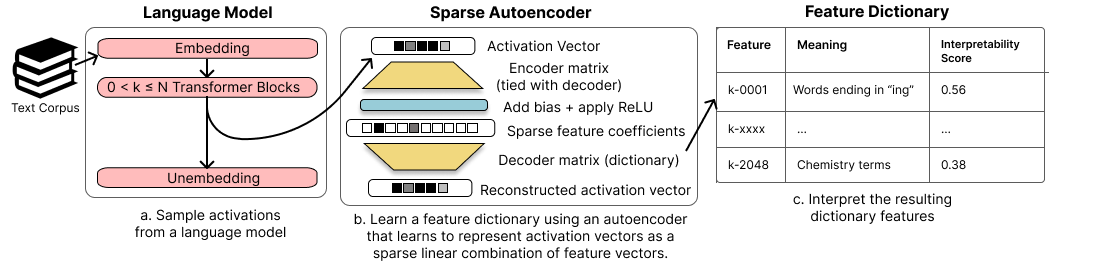
\includegraphics[width=1\textwidth]{images/sparse_coding_overview_1309.png}
    \caption{An overview of our method. We a) sample the internal activations of a language model, either the residual stream, MLP sublayer, or attention head sublayer; b) use these activations to train a neural network, a sparse autoencoder whose weights form a feature dictionary; c) interpret the resulting features with techniques such as OpenAI's autointerpretability scores.}
    \label{fig:overview}
\end{figure}
